\begin{tcolorbox}[
    colback=SkyBlue!5,
    colframe=blue!20,
    boxrule=1pt,
    arc=2pt,
    width=\textwidth,
    boxsep=5pt,
    left=5pt,
    right=5pt,
    top=5pt,
    bottom=5pt
]

\noindent
\begin{minipage}[b]{0.65\textwidth}
\begin{example}
Consider the program  
\begin{equation*}
  \tag{\textsc{r+r+r}}
  \label{ex:r+r+r}
  \inarr{ \textcolor{Red}{\readInst{a_1}{x}} }{ \textcolor{blue}{\readInst{a_2}{x}} }{ \textcolor{Dandelion!40!black}{\readInst{a_3}{x}} }
\end{equation*}

There is exactly one maximal execution: all reads read from $\init$.
The transition system $\mathcal{T}(\text{\textsc{r+r+r}})$ is a DAG with exactly one maximal execution.
\textbf{Algorithm K} estimates 6 executions, one for each ordering of the threads.
In general, if there were $n$ reads, \textbf{Algorithm K} would estimate $n!$ executions. \qed
\end{example}
\end{minipage}%
\hfill
\begin{minipage}[b]{0.40\textwidth}
\centering
\vspace{0pt}
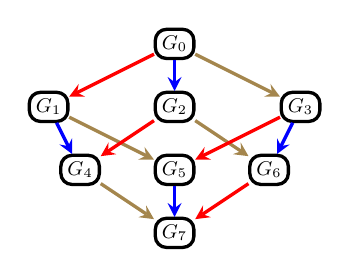
\begin{tikzpicture}[
    scale=0.8,
    transform shape,
    >=stealth,
    node distance=2.2cm and 2.5cm,
    hypernode/.style={draw, rectangle, rounded corners=4pt, very thick, inner sep=3pt, font=\small\bfseries},
    edge label/.style={midway, very thick,
    fill=white, font=\footnotesize, inner sep=1pt},
    edge-t1/.style={->, very thick, Red},
    edge-t2/.style={->, very thick, blue},
    edge-t3/.style={->, very thick, Dandelion!60!black}
]

% Top layer: G0
\node[hypernode] (G0) at (0,0) {$G_0$};

% Second layer
\node[hypernode] (G1) at (-2,-1) {$G_1$};
\node[hypernode] (G2) at (0,-1) {$G_2$};
\node[hypernode] (G3) at (2,-1) {$G_3$};

% Third layer
\node[hypernode] (G4) at (-1.5,-2) {$G_4$};
\node[hypernode] (G5) at (0,-2) {$G_5$};
\node[hypernode] (G6) at (1.5,-2) {$G_6$};

% Last layer
\node[hypernode] (G7) at (0,-3) {$G_7$};

% Edges from G0
\draw[edge-t1] (G0) -- (G1);
\draw[edge-t2] (G0) -- (G2);
\draw[edge-t3] (G0) -- (G3);

% Edges from G1
\draw[edge-t2] (G1) -- (G4);
\draw[edge-t3] (G1) -- (G5);

% Edges from G2
\draw[edge-t1] (G2) -- (G4);
\draw[edge-t3] (G2) -- (G6);

% Edges from G3
\draw[edge-t1] (G3) -- (G5);
\draw[edge-t2] (G3) -- (G6);

% Edges to G7
\draw[edge-t3] (G4) -- (G7);
\draw[edge-t2] (G5) -- (G7);
\draw[edge-t1] (G6) -- (G7);

\end{tikzpicture}
\label{hypergraph-rrr}


% \begin{figure}[t]
% \centering
% \resizebox{0.5\textwidth}{!}{ 
% \begin{tikzpicture}[
%     >=stealth,
%     node distance=1.4cm and 1.8cm,
%     event/.style={draw=none, font=\normalsize},
%     rf/.style={->, thick, dashed, green!60!black},
%     co/.style={->, thick, dotted, red!80!black},
%     hyper edge/.style={->, thick, blue!70!black},
%     graph box/.style={draw, rectangle, rounded corners=4pt, thick, minimum width=1.4cm, minimum height=1cm, inner sep=0.1cm, minimum size=0cm},
%     scale=0.65,
%     every node/.style={transform shape}
% ]

% % First row: G0, G1, G2, G3
% % G0
% \begin{scope}[xshift=-2cm, yshift=0cm, local bounding box=G0box]
%   \node[event] (g0i) {$\init$};
% \end{scope}
% \node[graph box, fit=(G0box)] (G0) {};

% % G1
% \begin{scope}[xshift=-6cm, yshift=-2cm, local bounding box=G1box]
%   \node[event] (g1i) {$\init$};
%   \node[event, below=0.7cm of g1i, xshift=-1.0cm] (g1r1) {$$\opr(x)$$};
%   \draw[->] (g1i) -- node[midway, left, font=\small] {$t_1$} (g1r1);
% \end{scope}
% \node[graph box, fit=(G1box)] (G1) {};

% % G2
% \begin{scope}[xshift=-2cm, yshift=-2cm, local bounding box=G2box]
%   \node[event] (g2i) {$\init$};
%   \node[event, below=0.7cm of g2i] (g2r2) {$$\opr(x)$$};
%   \draw[->] (g2i) -- node[midway, right, font=\small] {$t_2$}(g2r2);
% \end{scope}
% \node[graph box, fit=(G2box)] (G2) {};

% % G3
% \begin{scope}[xshift=2cm, yshift=-2cm, local bounding box=G3box]
%   \node[event] (g3i) {$\init$};
%   \node[event, below=0.7cm of g3i, xshift=1.0cm] (g3r3) {$$\opr(x)$$};
%   \draw[->] (g3i) -- node[midway, right, xshift=0.3cm, font=\small] {$t_3$}(g3r3);
% \end{scope}
% \node[graph box, fit=(G3box)] (G3) {};

% % Second row: G4, G5, G6
% % G4
% \begin{scope}[xshift=-6cm, yshift=-6cm, local bounding box=G4box]
%   \node[event] (g4i) {$\init$};
%   \node[event, below=0.7cm of g4i, xshift=-1.0cm] (g4r1) {$$\opr(x)$$};
%   \node[event, below=0.7cm of g4i] (g4r2) {$$\opr(x)$$};
%   \draw[->] (g4i) -- node[midway, left, font=\small] {$t_1$}(g4r1);
%   \draw[->] (g4i) -- node[midway, right, font=\small] {$t_2$}(g4r2);
% \end{scope}
% \node[graph box, fit=(G4box)] (G4) {};

% % G5
% \begin{scope}[xshift=-2cm, yshift=-6cm, local bounding box=G5box]
%   \node[event] (g5i) {$\init$};
%   \node[event, below=0.7cm of g5i, xshift=-1.0cm] (g5r1) {$$\opr(x)$$};
%   \node[event, below=0.7cm of g5i, xshift=1.0cm] (g5r3) {$$\opr(x)$$};
%   \draw[->] (g5i) -- node[midway, left, font=\small] {$t_1$}(g5r1);
%   \draw[->] (g5i) -- node[midway, right, xshift=0.3cm, font=\small] {$t_3$}(g5r3);
% \end{scope}
% \node[graph box, fit=(G5box)] (G5) {};

% % G6
% \begin{scope}[xshift=2cm, yshift=-6cm, local bounding box=G6box]
%   \node[event] (g6i) {$\init$};
%   \node[event, below=0.7cm of g6i] (g6r2) {$$\opr(x)$$};
%   \node[event, below=0.7cm of g6i, xshift=1.0cm] (g6r3) {$$\opr(x)$$};
%   \draw[->] (g6i) -- node[midway, right, font=\small] {$t_2$}(g6r2);
%   \draw[->] (g6i) -- node[midway, right, xshift=0.3cm, font=\small] {$t_3$}(g6r3);
% \end{scope}
% \node[graph box, fit=(G6box)] (G6) {};

% % Third row: G7
% % G7
% \begin{scope}[xshift=-2cm, yshift=-10cm, local bounding box=G7box]
%   \node[event] (g7i) {$\init$};
%   \node[event, below=0.7cm of g7i, xshift=-1.2cm] (g7r1) {$$\opr(x)$$};
%   \node[event, below=0.7cm of g7i] (g7r2) {$$\opr(x)$$};
%   \node[event, below=0.7cm of g7i, xshift=1.2cm] (g7r3) {$$\opr(x)$$};
%   \draw[->] (g7i) -- node[midway, left, font=\small] {$t_1$}(g7r1);
%   \draw[->] (g7i) -- node[midway, right, font=\small] {$t_2$}(g7r2);
%   \draw[->] (g7i) -- node[midway, right, xshift=0.3cm, font=\small] {$t_3$}(g7r3);
% \end{scope}
% \node[graph box, fit=(G7box)] (G7) {};

% % Hyperedges - First layer
% \draw[hyper edge] (G0) -- node[midway, above left, font=\small] {$t_1$} (G1);
% \draw[hyper edge] (G0) -- node[midway, above, font=\small] {$t_2$} (G2);
% \draw[hyper edge] (G0) -- node[midway, above right, font=\small] {$t_3$} (G3);

% % Hyperedges - Second layer
% \draw[hyper edge] (G1) -- node[midway, above left, font=\small] {$t_2$} (G4);
% \draw[hyper edge] (G1) -- node[midway, above right, font=\small] {$t_3$} (G5);
% \draw[hyper edge] (G2) -- node[midway, above left, font=\small] {$t_1$} (G4);
% \draw[hyper edge] (G2) -- node[midway, above right, font=\small] {$t_3$} (G6);
% \draw[hyper edge] (G3) -- node[midway, above left, font=\small] {$t_1$} (G5);
% \draw[hyper edge] (G3) -- node[midway, above right, font=\small] {$t_2$} (G6);

% % Hyperedges - Third layer
% \draw[hyper edge] (G4) -- node[midway, above left, font=\small] {$t_3$} (G7);
% \draw[hyper edge] (G5) -- node[midway, above, font=\small] {$t_2$} (G7);
% \draw[hyper edge] (G6) -- node[midway, above right, font=\small] {$t_1$} (G7);
% \end{tikzpicture}
% }
% \caption{The meta-graph of the \cref{ex:r+r+r}}
% \label{fig:rrr}
% \end{figure}

%%%%%%%%%%%% Hyper Node Graphs
% \begin{figure}
% \centering
% \begin{tikzpicture}[
%     >=stealth,
%     node distance=1.4cm and 1.8cm,
%     event/.style={draw=none, font=\small},
%     rf/.style={->, thick, dashed, green!60!black},
%     co/.style={->, thick, dotted, red!80!black},
%     ->, thick
% ]

% % First row:

% %G0
% \begin{scope}[xshift=0cm, yshift=0cm]
%   \node[event] (g0i) {$\init$};
%   \node[below=1.2cm of g0i] {(G0)};
% \end{scope}

% %G1
% \begin{scope}[xshift=3cm, yshift=0cm]
%   \node[event] (g1i) {$\init$};
%   \node[event, below=0.7cm of g1i, xshift=-1.2cm] (g1r1) {$$\opr(x)$$};
%   \draw[->] (g1i) -- node[midway, left] {$t_1$} (g1r1);
%   \node[below=1.2cm of g1i] {(G1)};
% \end{scope}

% %G2
% \begin{scope}[xshift=6cm, yshift=0cm]
%   \node[event] (g2i) {$\init$};
%   \node[event, below=0.7cm of g2i] (g2r2) {$$\opr(x)$$};
%   \draw[->] (g2i) -- node[midway, right] {$t_2$}(g2r2);
%   \node[below=1.2cm of g2i] {(G2)};
% \end{scope}

% %G3
% \begin{scope}[xshift=9cm, yshift=0cm]
%   \node[event] (g3i) {$\init$};
%    \node[event, below=0.7cm of g3i, xshift=1.2cm] (g3r3) {$$\opr(x)$$};
%   \draw[->] (g3i) -- node[midway, right, xshift=0.3cm] {$t_3$}(g3r3);
%   \node[below=1.2cm of g3i] {(G3)};
% \end{scope}

% %Second Row:

% %G4
% \begin{scope}[xshift=0cm, yshift=-2.5cm]
%   \node[event] (g4i) {$\init$};
%   \node[event, below=0.7cm of g4i, xshift=-1.2cm] (g4r1) {$$\opr(x)$$};
%   \node[event, below=0.7cm of g4i] (g4r2) {$$\opr(x)$$};
%   \draw[->] (g4i) -- node[midway, left] {$t_1$}(g4r1);
%   \draw[->] (g4i) -- node[midway, right] {$t_2$}(g4r2);
%   \node[below=1.2cm of g4i] {(G4)};
% \end{scope}

% % %G5
% \begin{scope}[xshift=3cm, yshift=-2.5cm]
%   \node[event] (g5i) {$\init$};
%   \node[event, below=0.7cm of g5i, xshift=-1.2cm] (g5r1) {$$\opr(x)$$};
%   \node[event, below=0.7cm of g5i, xshift=1.2cm] (g5r3) {$$\opr(x)$$};
%   \draw[->] (g5i) -- node[midway, left] {$t_1$}(g5r1);
%   \draw[->] (g5i) -- node[midway, right, xshift=0.3cm] {$t_3$}(g5r3);
%   \node[below=1.2cm of g5i] {(G5)};
% \end{scope}

% %G6
% \begin{scope}[xshift=6cm, yshift=-2.5cm]
%   \node[event] (g6i) {$\init$};
%   \node[event, below=0.7cm of g6i] (g7r2) {$$\opr(x)$$};
%   \node[event, below=0.7cm of g6i, xshift=1.2cm] (g7r3) {$$\opr(x)$$};
%   \draw[->] (g6i) -- node[midway, right] {$t_2$}(g7r2);
%   \draw[->] (g6i) -- node[midway, right, xshift=0.3cm] {$t_3$}(g7r3);
%   \node[below=1.2cm of g6i] {(G6)};
% \end{scope}

% %G7
% \begin{scope}[xshift=9cm, yshift=-2.5cm]
%   \node[event] (g7i) {$\init$};
%   \node[event, below=0.7cm of g7i, xshift=-1.2cm] (g7r1) {$$\opr(x)$$};
%   \node[event, below=0.7cm of g7i] (g7r2) {$$\opr(x)$$};
%   \node[event, below=0.7cm of g7i, xshift=1.2cm] (g7r3) {$$\opr(x)$$};
%   \draw[->] (g7i) -- node[midway, left] {$t_1$}(g7r1);
%   \draw[->] (g7i) -- node[midway, right] {$t_2$}(g7r2);
%   \draw[->] (g7i) -- node[midway, right, xshift=0.3cm] {$t_3$}(g7r3);
%   \node[below=1.2cm of g7i] {(G7)};
% \end{scope}
% \end{tikzpicture}
% \caption{The meta-graph of the RRR example}
% \label{meta-graph-rrr}
% \end{figure}

% %%%%%%%%%%% Abstract Hyper-graph
% \begin{figure}
% \centering
% \begin{tikzpicture}[
%     >=stealth,
%     node distance=2.2cm and 2.5cm,
%     hypernode/.style={draw, rectangle, rounded corners=4pt, thick, minimum width=1.4cm, minimum height=1cm, font=\small\bfseries},
%     edge label/.style={midway, fill=white, font=\footnotesize, inner sep=1pt}
% ]

% % Top layer: G0
% \node[hypernode] (G0) at (0,0) {G0};

% % Second layer
% \node[hypernode] (G1) at (-3,-2) {G1};
% \node[hypernode] (G2) at (0,-2) {G2};
% \node[hypernode] (G3) at (3,-2) {G3};

% % Third layer
% \node[hypernode] (G4) at (-2.5,-4.2) {G4};
% \node[hypernode] (G5) at (0,-4.2) {G5};
% \node[hypernode] (G6) at (2.5,-4.2) {G6};

% % Last layer
% \node[hypernode] (G7) at (0,-6.4) {G7};

% % Edges from G0
% \draw[->] (G0) -- (G1);
% \draw[->] (G0) -- (G2);
% \draw[->] (G0) -- (G3) ;

% % Edges from G1
% \draw[->] (G1) -- (G4);
% \draw[->] (G1) -- (G5);

% % Edges from G2
% \draw[->] (G2) -- (G4);
% \draw[->] (G2) -- (G6);

% % Edges from G3
% \draw[->] (G3) -- (G5);
% \draw[->] (G3) -- (G6);

% % Edges to G7
% \draw[->] (G4) -- (G7) ;
% \draw[->] (G5) -- (G7) ;
% \draw[->] (G6) -- (G7) ;

% \end{tikzpicture}
% \caption{Abstract hypergraph for the RRR example}
% \label{hypergraph-rrr}
% \end{figure}

\end{minipage}%
\end{tcolorbox}
